There are in general two types of thresholding that exist to binarize an image (create its mask): global and local.

\textbf{Global thresholding} is a an algorithm that simply choses one threshold $T$ for the whole histogram of the image. All pixels that are smaller than this threshold $x_{i,j} < T$ are assigned to be of class $0$ (background) and all pixels that are larger than this threshold $x_{i,j} > T$ are assigned to be of class $1$ (foreground). It is very difficult to find a good threshold manually that would work out for all the images, especially in this case, when the brightness does differ not only between the images, but also within the image itself (light gradient in Figure \ref{fig:lightning_conditions}). To find a good threshold automatically (at least to some extect) \cite{digital_image_book} proposed the following algorithm:

\begin{algorithm}
  \caption{Global thresholding}
  \begin{algorithmic}
    \item 1. Select an initial estimate for $T$.
    \item 2. Segment the image using T. This will produce 2 groups of pixels $G_1$ (all pixels $x_i > T$) and $G_2$ (all pixels $x_i < T$).  
    \item 3. Computer the average gray values $\mu_1$ and $\mu_2$ for the pixels in  regions $G_1$ and $G_2$.
    \item 4. Compute a new threshold value 
        $T' = \frac{\mu_1 + \mu_2}{2}$
    \item 5. Repeat steps 2-4 until difference in the change of value $T$ is smaller that a predefined parameter.
  \end{algorithmic}
  \label{alg:global-thresholding}
\end{algorithm}

Nevertheless, it is not obvious how to preselect an initial threshold in step 1. There are several options here, however keep in mind that there is also no single best solution among them. For example, when an assumption that the foreground occupies approximately the same area as the background holds, than initial threshold $T$ should be chosen to be an average gray level and etc.

After trying out many different global threshold approaches, it has been derived that a \textit{global minimum thresholding} is the best one. It is implemented in \textit{skimage.filters} and according to the documentation (\cite{global_thresh}) works in the following way: it assumes that the histogram $p = (p_0, \ldots, p_{M})$ of the image is bimodal, meaning that it has two clearly defined peaks (background and foreground). Afetrwards the histogram is iteratively smoothed using a running average of size $k=3$. The points on the histogram are updated with the value $a_k$ from Equation \ref{eq:SMA} until only 2 local maximas ($a_l$ and $a_r$) are left. 
\begin{equation}
    a_k = \frac{1}{k}\sum_{i=n-k + 1}^{n}p_i
\label{eq:SMA}
\end{equation}
Then the threshold is taken as the minimum between the two local maximas:
\begin{equation}
    a_l \leq T \leq a_r
\end{equation}

One clear downside of this approach though is that images which histograms have very unequal peaks or a broad and flat valley will be unsuitable for this method (\cite{thresholding_skimage}).

\begin{figure}[htb]
	\begin{center}
		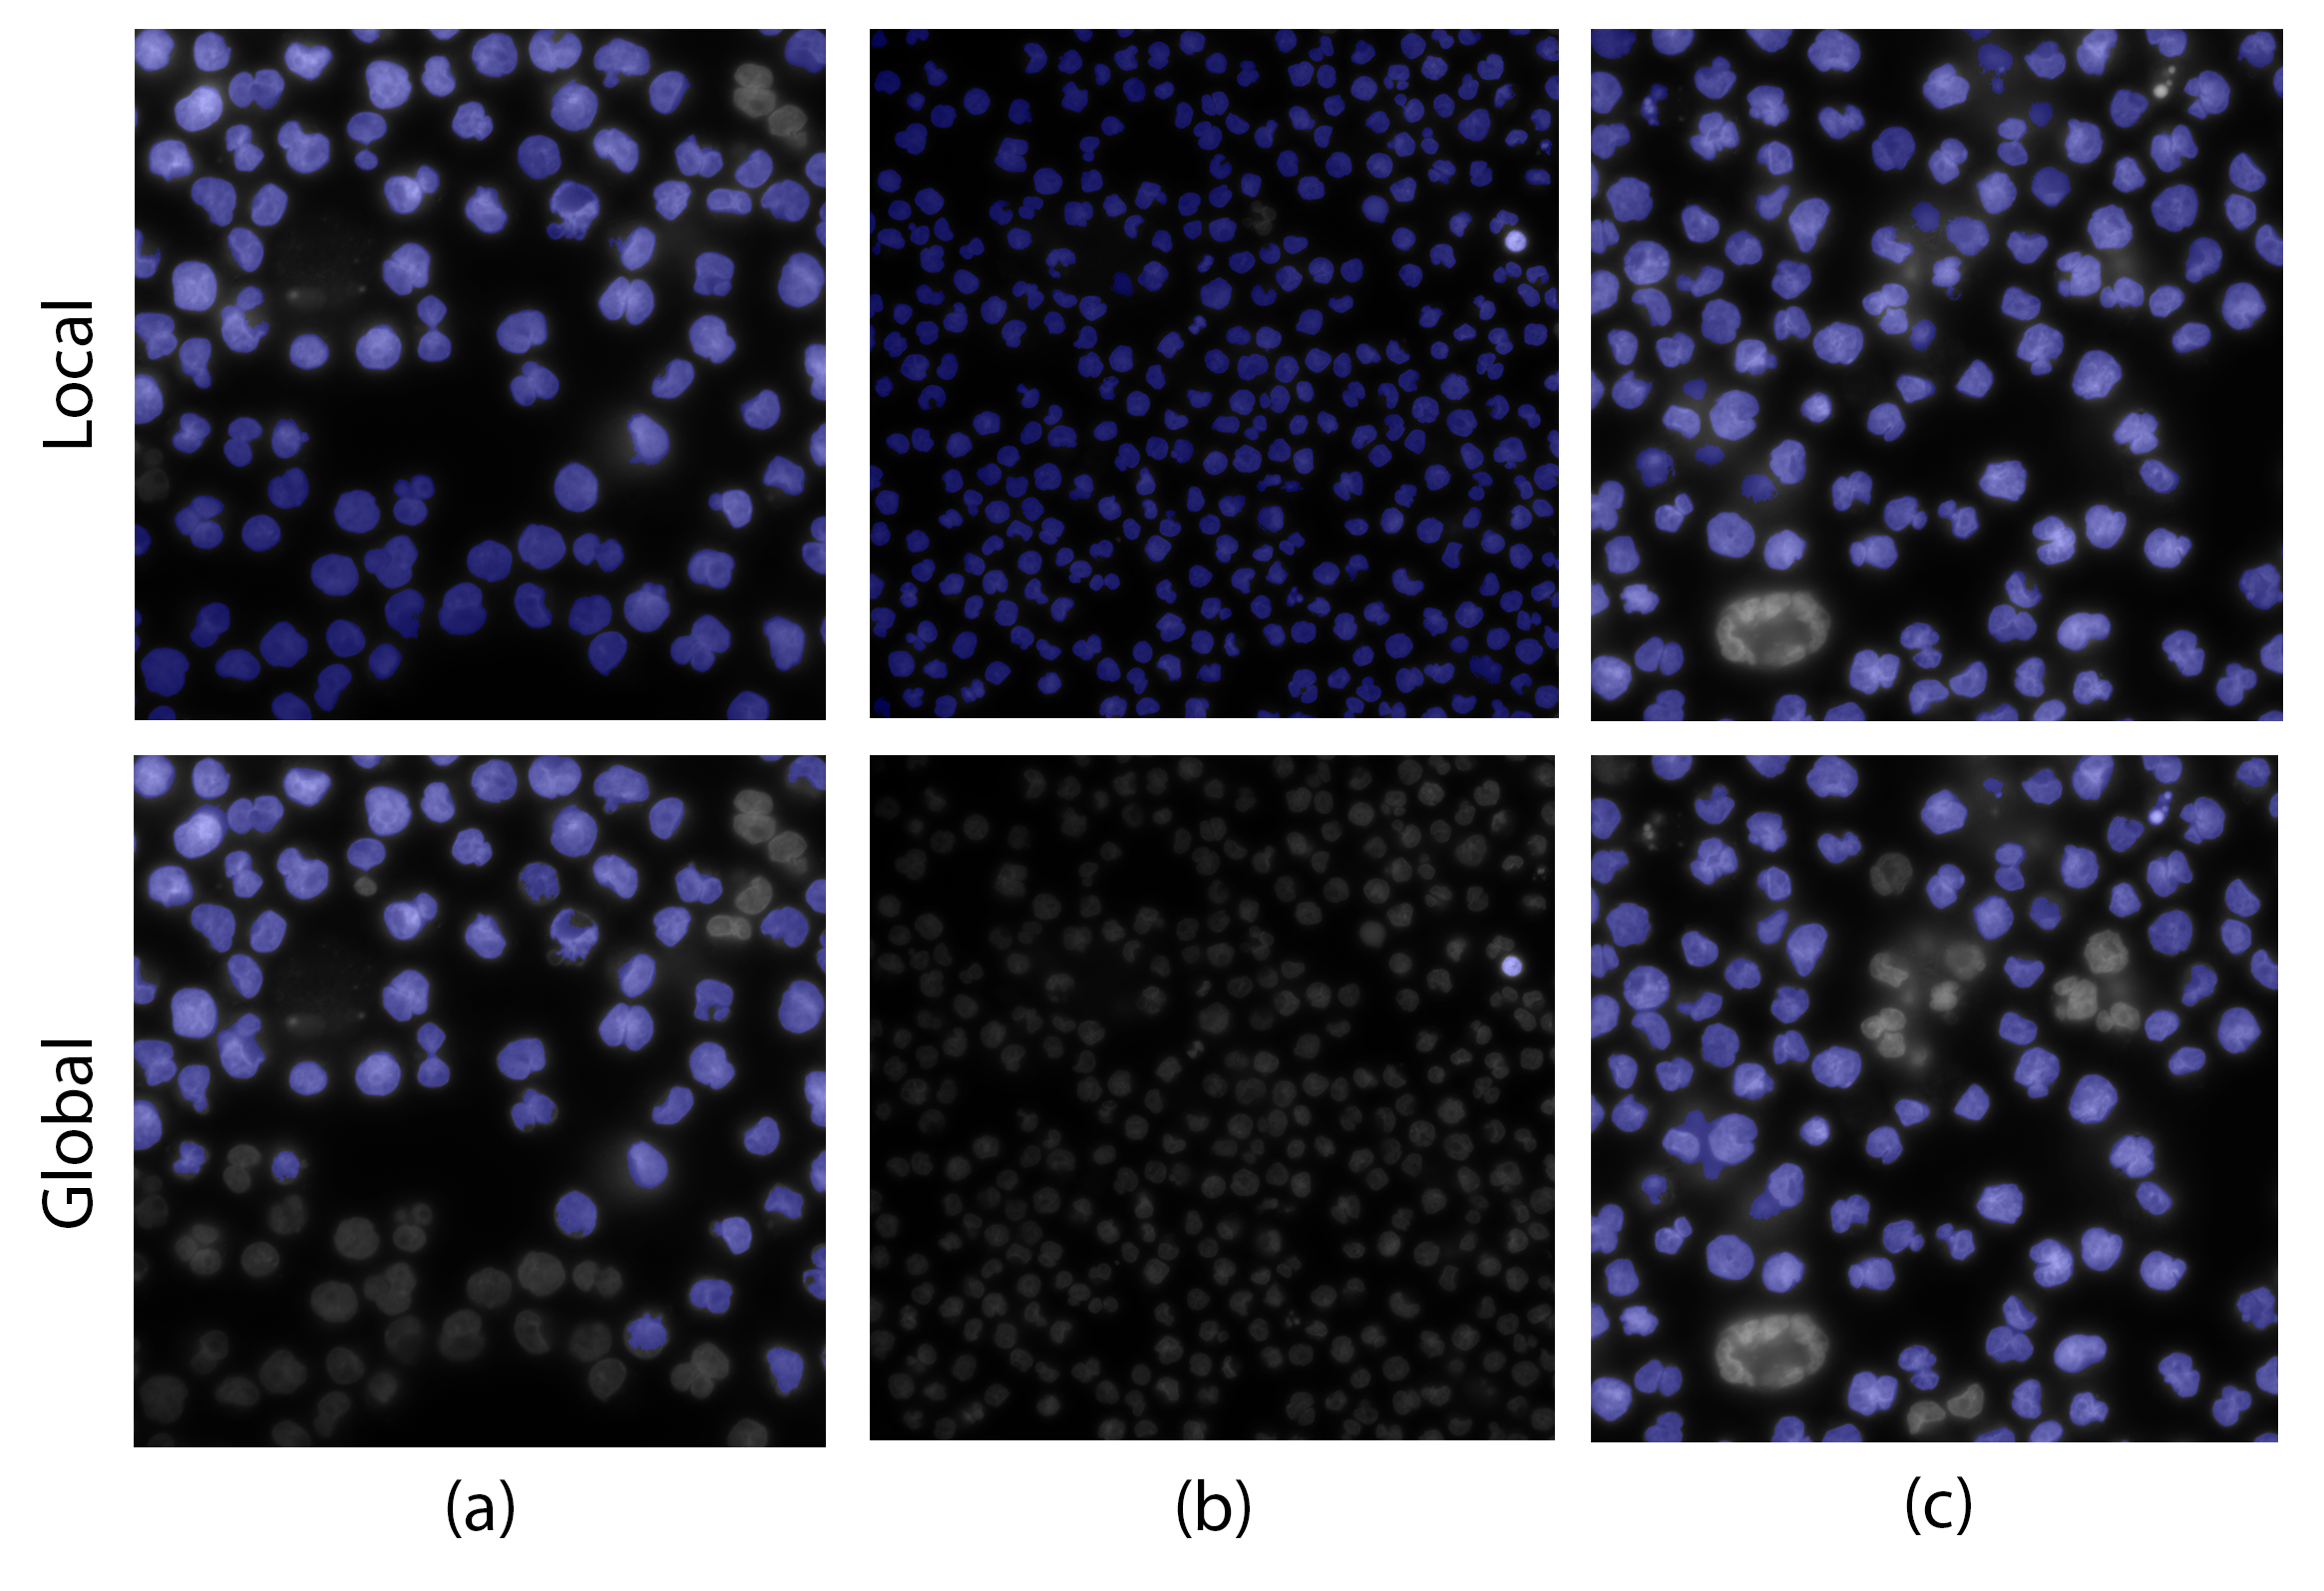
\includegraphics[width=0.6\linewidth]{bilder/difficult-lightning/local-vs-global.png}
		\caption[Local vs. global thresholding]%
        {Local vs. global thresholding. A compasion of the results of two approaches for three lightning situations: (a) --- gradient in image illumination; (b) --- overexposure of one cell resulting in underexposure of all other celss; (c) --- normal conditions.}\label{fig:thresholding-bad-conditions}
	\end{center}
\end{figure}

Unfortunately this method did not perfom well even for the images that have an equal amount of foreground and background. And the reason for that is a mentioned above non-uniform illumination within the images. For visual comparison of global thresholding applied to difficult images see Figure \ref{fig:thresholding-bad-conditions}a, b, c Global. \ref{fig:thresholding-bad-conditions}c is an image with equal brightness level, however even there some mistakes do appear.

However, there is another better approach that performs well in such conditions: \textbf{local thresholding}. For nuclei segmentation exactly this algorithm was chosen. It is implemented in \textit{skimage.filters} and can be used in the following way:

\begin{lstlisting}
  skimage.filters.local_threshold(img, block_size=7, method='gaussian', offset=0)
\end{lstlisting}

The main idea behind it is the following: instead of selecting one threshold for the whole image (global one), one can select several thresholds for each local region with a predefined size. The comparison between global and local thresholding is presented in Figure \ref{fig:thresholding-bad-conditions}, where (a), (b) denote exteme corruption cases and (c) represents a normal illumination.

"The threshold value is the weighted mean for the local neighborhood of a pixel subtracted by a constant (\cite{digital_image_book})". With the image size of $2136 \times 2136$, the local neighborhood (or a \textit{block\_ size}) by experimenting with different values was chosen equal to $111$. The default \textit{method} used on for local thresholding is \textit{gaussian}, \textit{offset} value is a constant that will be subtracted from weighted mean of neighborhood during the calculation of the local threshold, by default this value is $0$ \cite{local_thresholding}.

Let $z$ be a random variable that quantifies a gray-level value of the pixel, then the histogram of the image is a probability density function (PDF) $p(z)$. Since we assume that the image contains a background and a foreground, then this PDF is a mixture of two densities $p_1(z)$ and $p_@(z)$ weighted by the relative areas of these two classes (their number of pixels) $P_1$ and $P_2$. Then 

\begin{equation}
    p(z) = P_1 p_1(z) + P_2 p_2(z)
\end{equation}

By assuming Gauassian model for both $p_1(z)$ and $p_2(z)$, one gets a Gaussian Mixture Model (GMM). Since we have assumed that each pixel can be asssigned to either a background of foreground only, $P_1 + P_2 = 1$ must hold. 

\begin{figure}[htb]
	\begin{center}
		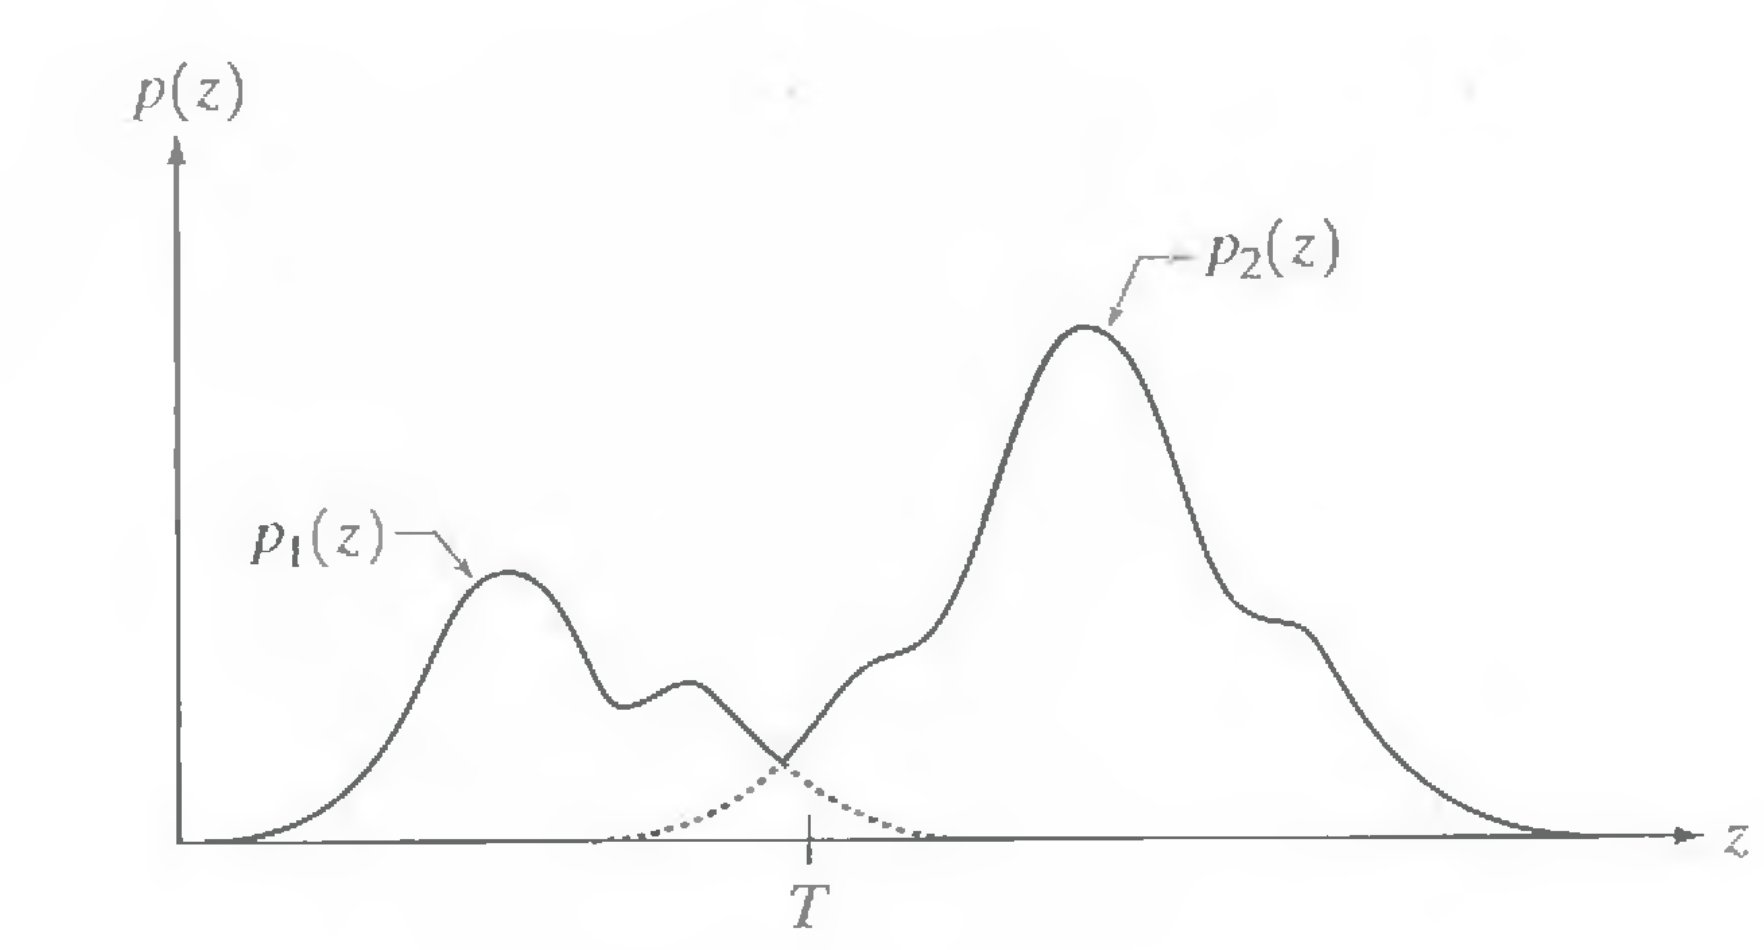
\includegraphics[width=0.8\linewidth]{bilder/Gonzalez.png}
		\caption[Histogram as a probability density function]%
        {Histogram as a probability density function. Taken from \cite{digital_image_book}}\label{fig:gmm}
	\end{center}
\end{figure}

Probability to falsely classify an background pixel as a foreground then is:

\begin{equation}
    E_1(T) = \int_{-\infty}^T{p_2(z) \, dz}
\end{equation}

And probability to falsely classify a foreground pixel as a background then is:

\begin{equation}
    E_2(T) = \int_T^{+\infty}{p_1(z) \, dz}
\end{equation}

The overall error is:

\begin{equation}
    E(T) = P_1E_1(T) + P_2E_2(T)
\end{equation}

By differentiating $E(T)$ wrt. to $T$ and equating the result to zero the optimal solution will be:

\begin{equation}
    P_1p_1(T) = P_2p_2(T)
\end{equation}

Since Gaussian distributions have been assumed, it will hold that:
\begin{equation}
    p(z) = \frac{P_1}{\sqrt{2\pi} \sigma_1}e^{-\frac{(z-\mu_1)^2}{2\sigma_1^2}} + \frac{P_2}{\sqrt{2\pi} \sigma_2}e^{-\frac{(z-\mu_2)^2}{2\sigma_2^2}}
\end{equation}

With $\mu_i$ and $\sigma_i^2$ for $i \in \{1, 2\}$ being the mean and variance of the Gaussian distribution $p_i(z)$. This results in the following solution for $T$:
\begin{equation}
    \begin{split}
        &AT^2 + BT + C = 0 \\
        &A = \sigma_1^2 + \sigma_2^2 \\
        &B = 2(\mu_1 \sigma_1^2 - \mu_2 \sigma_2^2) \\
        &C = \sigma_1^2 \mu_2^2 - \sigma_2^2 \mu_1^2 + 2\sigma_1^2 2\sigma_2^2ln\left(\frac{\sigma_2P_1}{\sigma_1P_2}\right)
    \end{split}
\end{equation}

To escape two optimal solutions of the quadratic equation, it may be assumed that $\sigma_1 = \sigma_2 = \sigma$ and then:

\begin{equation}
    T = \frac{\mu_1 + \mu_2}{2} + \frac{\sigma^2}{\mu_1 - \mu_2}ln\left(\frac{P_2}{P_1}\right)
\end{equation}

Such threshold search is then applied to all of the subregions of the image with overlaps. Thresholds are calculated only for the regions that contain two clear peaks in their histograms and interpolated to the other pixels from the regions that do not contain them. If the subregions does not contain two peaks, it simply means that there is no foreground or background object on it. 

\begin{table}[htb]
  \centering
      \begin{tabular}{||c c||} 
       \hline
       Local Threshold & Global Threshold \\ [0.5ex] 
       \hline\hline
       0.3 sec & 17 sec  \\ 
       \hline
      \end{tabular}
      \caption{Threshold runtime}
      \label{table:threshold-timing}
  \end{table}
  
Of course local thresholding approach has a longer runtime time (see Table \ref{table:threshold-timing}). Therefore when the inference speed is crutial one can still use \textit{global minimum thresholding}. It does performs visually a bit worse that a local threshold (especially for the extreme corrupted cases), however for the normal conditions the performance is quite similar ot the local thresholding (Figure \ref{fig:thresholding-bad-conditions}c). One should also keep in mind, that after the model is trained due to its generalization ability the gradient in intensities or overexposure will not be present anymore, as it is related to the image acquisition technique and does not depend on the DIC image itself.


